\documentclass[]{article}
\usepackage[T1]{fontenc}
\usepackage[icelandic]{babel}
\usepackage{lipsum}
\usepackage{natbib}

\input{../shorthandCommon}

%opening
\title{Vélabrögð}
\author{Helga Ingimundardóttir}

\begin{document}

\maketitle

%\begin{abstract}\end{abstract}

\section{Inngangur}
Í stuttu máli snýst verkefnið um að læra að bera kennsl á góðar lausnir. 
Ég hef einskorðað verkefnið við tilviksrannsókn á verkniðurröðun á vélum (JSP, 
e. job-shop scheduling problem) 
sem felst í því að þurfa að gera raðbundnar ákvarðanir um hvaða verk eigi 
að vera afgreitt næst, þar sem þau eru að keppast um sömu aðföngin.
Í raun má útvíkka aðferðafræðina til hvers kyns strjála bestun. 

Hugmyndina að rannsókninni kviknaði þegar ég var að vinna í raunhæfu verkefni í 
aðgerðagreiningu í grunnnámi mínu. Um var að ræða bestun á verkniðurröðun fyrir 
Össur. Í eðli sínu er verkniðurröðun einfalt verkefni, og skipar stóran sess 
hjá framleiðslufyrirtækjum en stærðargráðan á vandamálinu gerir það að verkum 
að oft er erfitt að leysa verkefnið með nákvæmum aðferðum. 
Þetta voru mín fyrstu kynni af því að þurfa að sætta mig við einhverja lausn 
sem var ekki endilega hin fræðilega ,,besta'' lausn. 
Hér koma brjóstvitsaðferðir (e. heuristics) eða ,,þumalputtareglur'' sterkar 
inn, en þá er stóra spurningin hvernig má koma á sjálfvirkni í því ferli?

\section{Verkniðurröðun á vélar}
Gerum ráð fyrir að við höfum $n\times m$ JSP, 
þar sem $n$ verk, $\mathcal{J}=\{J_j\}_{j=1}^n$, 
eiga að vera afgreidd á $m$ vélum, $\mathcal{M}=\{M_a\}_{a=1}^m$. 
Verkefnin þurfa að vera afgreidd í tiltekinni röð, þ.e. sérhvert verk $J_j$ 
þarf að fylgja runu af $m$ aðgerðum 
$\vsigma_j=\{\sigma_{j1},\sigma_{j2},\dotsc,\sigma_{jm}\}$. 
Rétt er að taka fram að verk getur ekki hafist handa á næstu vél fyrr en það 
hefur lokið núverandi aðgerð. 
Þar að auki getur sérhver vél aðeins meðhöndlað eitt verk í einu. 
Viðbættar skorður sem eru oft teknar til greina eru sleppitími og útgáfutími, 
en þeir eru ekki til skoðunar hér.
Markfallið er að tímasetja öll verk þannig að lágmarka skal hámarks heildartíma 
(e. makespan), $C_{\max}$. 

\begin{figure}\centering
    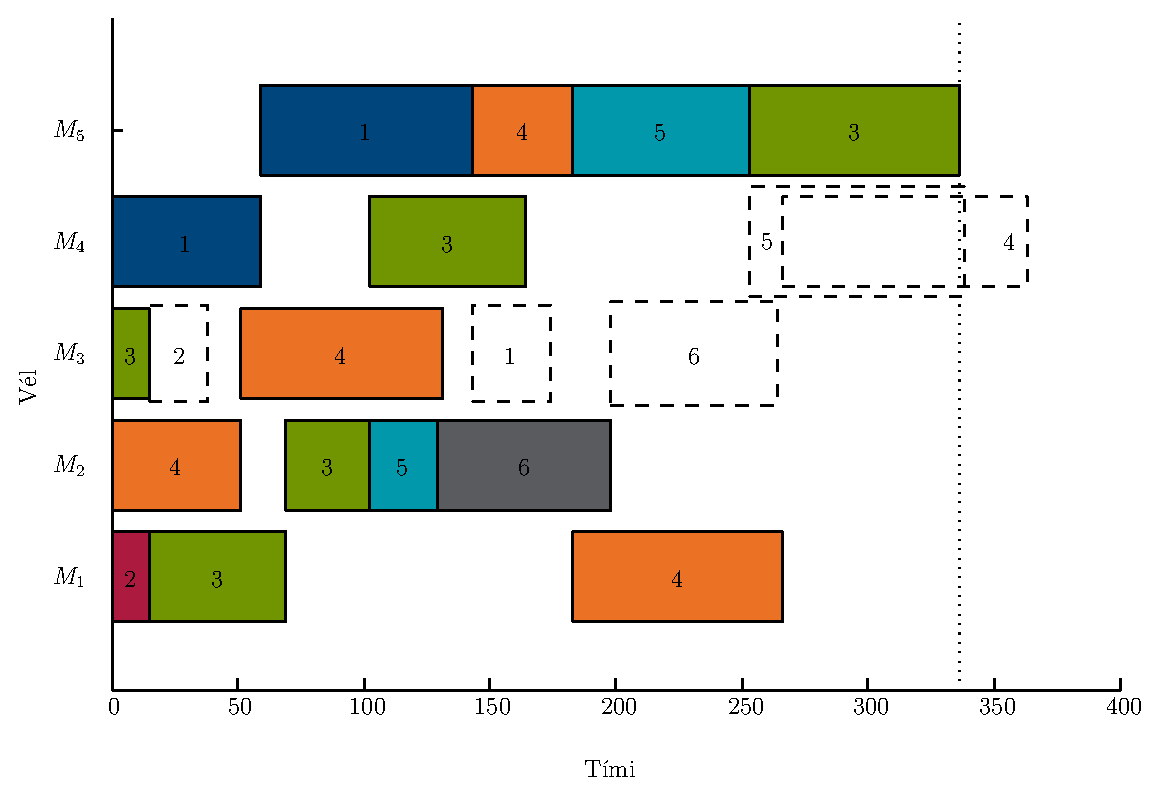
\includegraphics[width=0.8\textwidth]{figures/jssp_example.eps}
    \caption[Gantt rit af ókláraðri JSP stundaskrá]{Gantt rit af ókláraðri JSP 
    stundaskrá eftir 15 aðgerðir: heilir kassar tákna $\vchi$ og kassar með 
    brotalínu tákna $\mathcal{L}^{(16)}$. 
    Núverandi heildartími, $C_{\max}$, er gefinn upp sem punktalína.}
    \label{fig:jssp:example}
\end{figure}

Brjóstvitsaðferðir fyrir tímaáætlanir eru yfirleitt uppbyggingar- eða 
umbætunaralgrím.
Umbætunaralgrím byrja á fulbúinni lausn og reynir að finna sambærilegar, en 
betri lausnir. 
Uppbyggingaralgrím byrja með tóma lausn og bæta við einu verki í einu þar til 
lausnin er fullbúin, og er það sú nálgun sem aðferðafræðin mín gengur út frá. 
Í þessu tilfelli þá eru yfirleitt röðunarreglur (DR, e. dispatching 
rules) sem ákvarða hvaða ókláraða verk verður valið næst. Það er ekki nóg að 
vita hvaða verkefni ætti að vera valið næst, 
heldur þarf líka að athuga hvar væri best að staðsetja það. 
Þar sem við viljum búa til samþjappaðar tímaáætlanir  þá setjum við verkið af 
stað um leið og það er laust. 
Skoðnum nú Gantt ritið á mynd \ref{fig:jssp:example} sem sýnir dæmi um 
$6\times5$ JSP þar sem verknúmerið er gefið inn í kassa og er breidd hans 
vinnslutími verksins, 
vélarnar eru á lóðrétta ásinum og lárétti ásinn segir til um tíma 
og er núverandi $C_{\max}$ gefið sem punktalína. 
Búið er að setja af stað 15 aðgerðir, nefnilega, 
\begin{eqnarray}
\vchi=\left(J_3,J_3,J_3,J_3,J_4,J_4,J_5,J_1,J_1,J_2,J_4,J_6,J_4,J_5,J_3\right),
\end{eqnarray}
þar af leiðandi eru ókláruð verkin eftirfarandi 
$\mathcal{L}=\{J_1,J_2,J_4,J_5,J_6\}$, sem lýsa þeim 5 mögulegu verkum sem geta 
verið afgreidd á tímapunkti $k=16$ (athugið að verk $J_3$ er fullklárað) -- 
þessi verk eru gefin upp með brotalínu og lýsa hvernig staðan gæti breyst. 
Við sjáum að $J_2$ getur verið staðsett á $M_3$ annaðhvort á milli  $J_3$ 
$J_4$, eða eftir $J_4$.  Ef $J_6$ hefði nú þegar verið afgreitt, þá myndi 
myndast rauf á milli þess og $J_4$, þ.a.l. myndast þriðji möguleikinn, þ.e. 
fyrir $J_2$ er sett eftir $J_6$. 
Uppbyggingaralgrímið þarf því að ákveða hvert þessara möguleika ætti að vera 
valið fyrir verkið og er það óháð röðunarreglunni sem er notuð. 
Mismunandi staðsetningaraðferðir geta verið skoðaðar, t.a.m. að velja þau rauf 
sem er minnsta (en nægjanlega stór) fyrir verkið. En grunnrannsóknir sýndu að 
slík nálgun gat í raun útilokað bestu lausn m.t.t. lágmarks heildartíma. 
En slík staða kom ekki upp ef við afgreiðum verkin um leið og þau berast. 

\section{Röðunarreglur}
Einfaldar röðunarreglur (SDR, e. single-based priority dispatching rule) 
(SDR), er fall af sérkennum verka/véla tímaáætlunarinnar. Sérkennin geta verið 
fastar eða breyst í takti við ferlið. Til dæmis getur forgangurinn byggst á 
eiginleikum vinnslutíma verkanna, 
\begin{description}
    \item[Minnsti vinnlutími (SPT, e. shortest immediate processing time)] 
    \hfill \\ gráðug aðferð sem klárar verk með minnsta vinnslutíma fyrst, 
    \item[Stærsti vinnslutími (LPT, e. longest immediate processing time)] 
    \hfill \\ gráðug aðferð sem klárar verk með stærsta vinnslutíma fyrst, 
    \item[Minnsta heildarvinna (LWR, e. least work remaining)] \hfill \\
    þar sem ásetningurinn er að klára verk sem eru komin langt á veg í 
    framvindu sinni, þ.e. að lágmarka verklistann $\mathcal{L}$,
    \item[Stærsta heildarvinna (MWR, e. most work remaining)] \hfill \\
    þar sem ásetningurinn er að flýta fyrir framvindu verka sem krefjast mikinn 
    vinnslutíma, og gefur því af sér jafnari framvidnu fyrir öll verk, aftur á 
    móti.
\end{description}
Þetta eru þær algengustu röðurnarreglur í starfi vegna einfaldleika þeirra og 
skilvirkni, en ótal fleiri reglur koma líka til greina. Yfirlit yfir 100 
sígildar röðunarreglur má finna í \citet{Panwalkar77}, en einnig er greinargóð 
lýsing á SDR eftir \citet{Haupt89}. 




\begin{figure}
    \includegraphics[width=\textwidth]{figures/{stepwise.6x5.Track.casescenario}.pdf}
    \caption{Mean best and worst case scenario over various trajectories.}
    \label{diff:case:track:jrnd:6x5}
\end{figure}

\begin{figure}
    \includegraphics[width=\textwidth]{figures/{stepwise.6x5.OPT.SDR}.pdf}
    \caption{Probability of SDR being optimal}
    \label{fig:diff:opt:SDR}
\end{figure}


          Problem Dimension    Q1    Q3
          j.rnd.6x5   j.rnd       6x5 19.91 47.21
          f.rnd.6x5   f.rnd       6x5 18.46 35.52


\bibliographystyle{unsrtnat}
\bibliography{../references}  
\end{document}



„Ég skoða ólíkar lausnir við verkniðurröðun og hvernig einkennisþættir, t.d. 
ónýttur tími á færibandi, breytast í gegnum framleiðsluferlið. Lausnir eru 
bornar saman tvær og tvær og ákvarðað hvort önnur sé betri en hin. Síðan er 
beitt reiknifræðilegum aðferðum til að yfirfæra þessa þekkingu á ný verkefni,“ 
segir Helga.


Hún segir áherslu sína í námi hafa færst frá hinu fræðilega til hins hagnýta og 
hún hafi heillast af reiknigreind, en það er aðferð sem notuð er til að finna 
tengsl á milli tveggja hluta sem menn koma ekki svo auðveldlega auga á. Til 
þess eru stundum notaðar ofurtölvur. „Reiknigreind er nánast töfrum líkust. Með 
því að rýna í sambærileg verkefni og nýta tölvutækni er hægt að öðlast alls 
konar fróðleik, t.a.m. torræða þekkingu eða tilfinningu þeirra sem hafa 
ígrundað árum saman verkefni sem eru sambærileg,“ segir Helga og nefnir sem 
dæmi stundatöflur fyrir skóla.

Helga segist líta svo á að sitt hlutverk sé að koma með sérfræðivitneskju inn í 
hönnunina hjá framleiðslufyrirtækjum og láta svo tölvur sjá um mesta erfiðið. Í 
því skyni er hún að hanna reiknirit en þau eru notuð í stærðfræði og 
tölvunarfræði við lausn vandamála. „Reikniritið lærir að gera greinarmun á 
„góðum“ og „slæmum“ lausnum. Því má segja að aðferðafræðin eigi erindi í 
sérhverju verkefni sem felur að einhverju leyti í sér bestun, en sá listi er 
ótæmandi,“ segir Helga að lokum.